\documentclass{standalone}

\usepackage
{
	tikz,
	pgfplots,
	verbatim,
	amssymb,
}


\usetikzlibrary
{
	arrows,
	patterns,
	angles,
	quotes,
	calc, 
	3d,
	backgrounds, 
	positioning
}

\begin{document}
	\pgfplotsset{
		compat=newest,
		every axis/.append style={
			width=10cm,
			axis x line=middle,
			axis y line=middle,
			enlargelimits=true,
			xlabel={$x$},
			xlabel style={below left, scale=1.5},
			ylabel={$y$},
			ylabel style={below right, scale=1.5},
			ymajorgrids=true,
			xmajorgrids=true,
			xticklabels={},
			yticklabels={},
			samples=1000,
			%grid style={thick},
			axis line style={thick},
			ticks=both,
			xtick={-100,-99,...,100},
			ytick={-100,-99,...,100},
			restrict y to domain=-100:100,
			set layers=standard,
			every major tick/.style={draw=none},
			every minor tick/.style={draw=none},
			domain=-20:20
	}}
	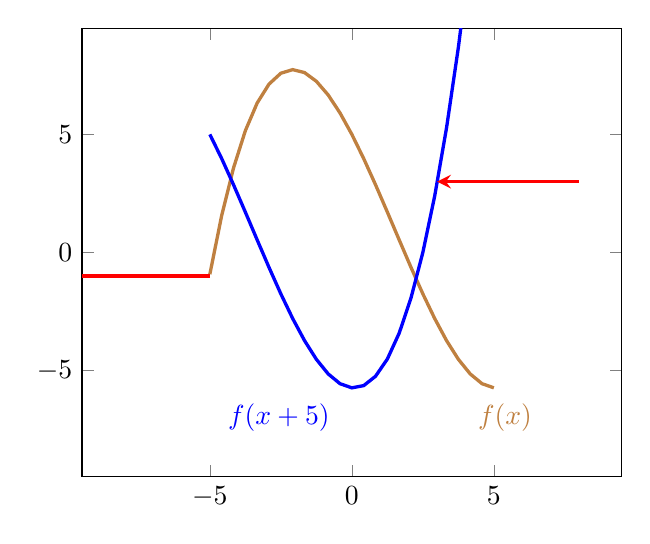
\begin{tikzpicture}[>=stealth, baseline={([yshift={-\ht\strutbox}]current bounding box.north)}]
		\begin{axis}[
			xmin=-9.5,xmax=9.5,
			ymin=-9.5,ymax=9.5]
			\addplot [brown,line width=1.2pt] {2/27*x^3-x^2/3-7/3*x+5};
			\addplot [blue,line width=1.2pt] {2/27*(x+5)^3-(x+5)^2/3-7/3*(x+5)+5};
			\draw (4.1,-6) node[anchor=north west, brown, fill=white] {$f(x)$};
			\draw (-4.7,-6) node[anchor=north west, blue, fill=white] {$f(x+5)$};
			\draw[<-, red, line width=1.2pt] (-10,-1) -- (-5,-1);
			\draw[<-, red, line width=1.2pt] (3,3) -- (8,3);
		\end{axis}
	\end{tikzpicture}
	
\end{document}